\documentclass{beamer}


\usepackage[utf8]{inputenc}
\usepackage[frenchb]{babel}
\usepackage{verbatim}
\usepackage{graphicx}
	\graphicspath{{figures/}}
\usepackage{caption}
\usepackage{subcaption}
\usepackage{color}

\usetheme{boxes}
\usecolortheme{beaver}
\beamertemplatenavigationsymbolsempty
\setbeamertemplate{title page}[default][colsep=-4bp,rounded=true]
\setbeamertemplate{sections/subsections in toc}[circle]
\setbeamertemplate{footline}[frame number]
\setbeamertemplate{itemize items}[circle]
\setbeamertemplate{itemize subitem}[square]
\setbeamertemplate{blocks}[rounded][shadow=false]
\setbeamercolor{block title}{bg=blue!40,fg=black}
\setbeamercolor{block body}{bg=blue!10,fg=black}




\definecolor{lightgreen}{rgb}{0.0,0.8,0.0}
\definecolor{lightblue}{rgb}{0.3,0.8,1.0}
\definecolor{lightred}{rgb}{0.874,0.180,0.105}
\definecolor{gray}{rgb}{0.4,0.4,0.4}
\definecolor{lightgray}{rgb}{0.8,0.8,0.8}
\definecolor{shadecolor}{rgb}{0.9,0.9,0.9}


\title{Inférence bayésienne adaptative pour la reconstruction de source en dispersion atmosphérique}
\author{Harizo Rajaona}
\institute{CrisTaL - CEA - Aria Technologies}
\date{21 novembre 2016}

\begin{document}
\AtBeginSection[]
{
	\begin{frame}
		\tableofcontents[currentsection]
		% Die Option [pausesections]
	\end{frame}
}
	
	
\begin{frame}
	\titlepage
\end{frame}
\begin{frame}
	\tableofcontents
\end{frame}

\section{Contexte et problématique}

% ===== Contexte (1) ================================================================
\begin{frame}
	\frametitle{Contexte}
	Les rejets \textbf{NRBC}\footnote{Nucléaires, Radiologiques, Biologiques, Chimiques} dans l'atmosphère peuvent être d'origine:
	\begin{itemize}
		\item accidentelle (fuite ou explosion sur un site industriel),
		\item malveillante (actes terroristes)
	\end{itemize}
	\begin{figure}
		\centering
		\begin{subfigure}[b]{0.33\textwidth}
			\centering
			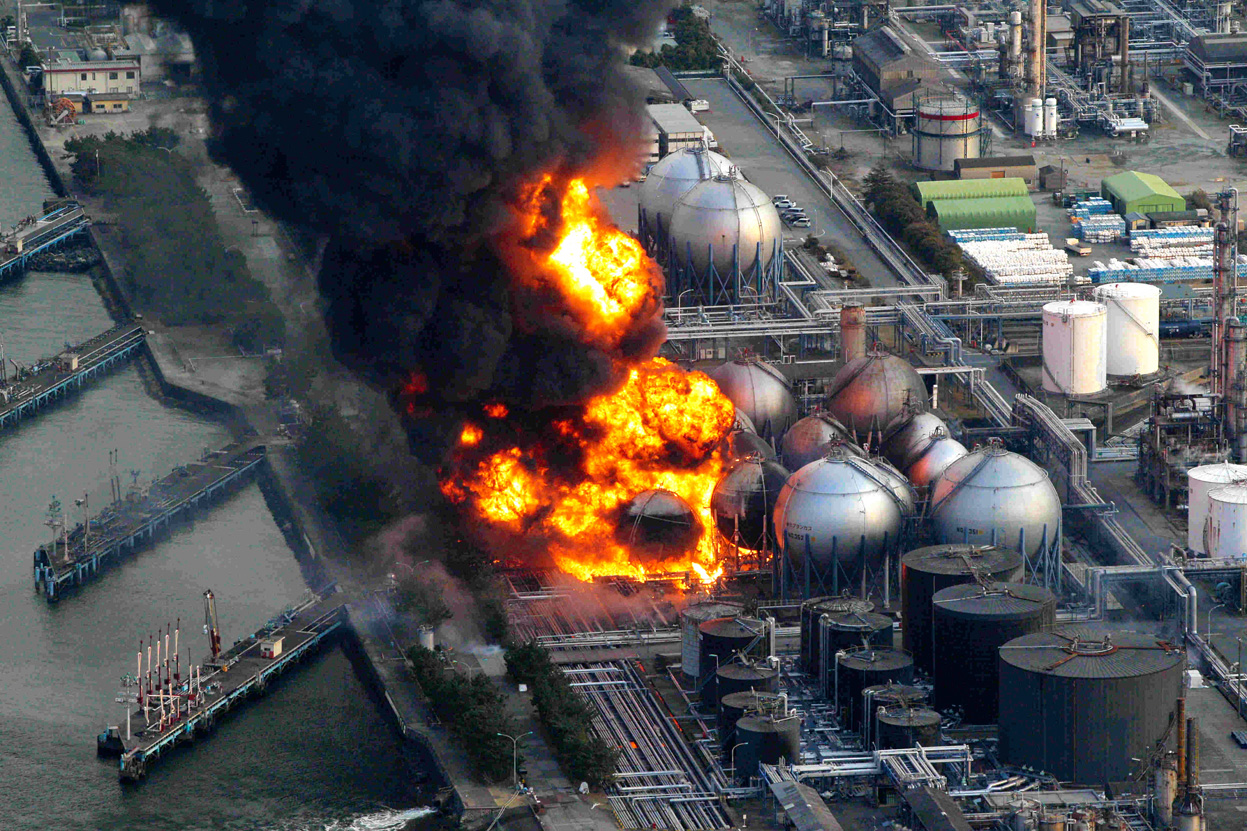
\includegraphics[width=\textwidth]{fukushima}
			\caption*{Fukushima (2011)}
		\end{subfigure}
		\hfill
		\begin{subfigure}[b]{0.3\textwidth}
			\centering
			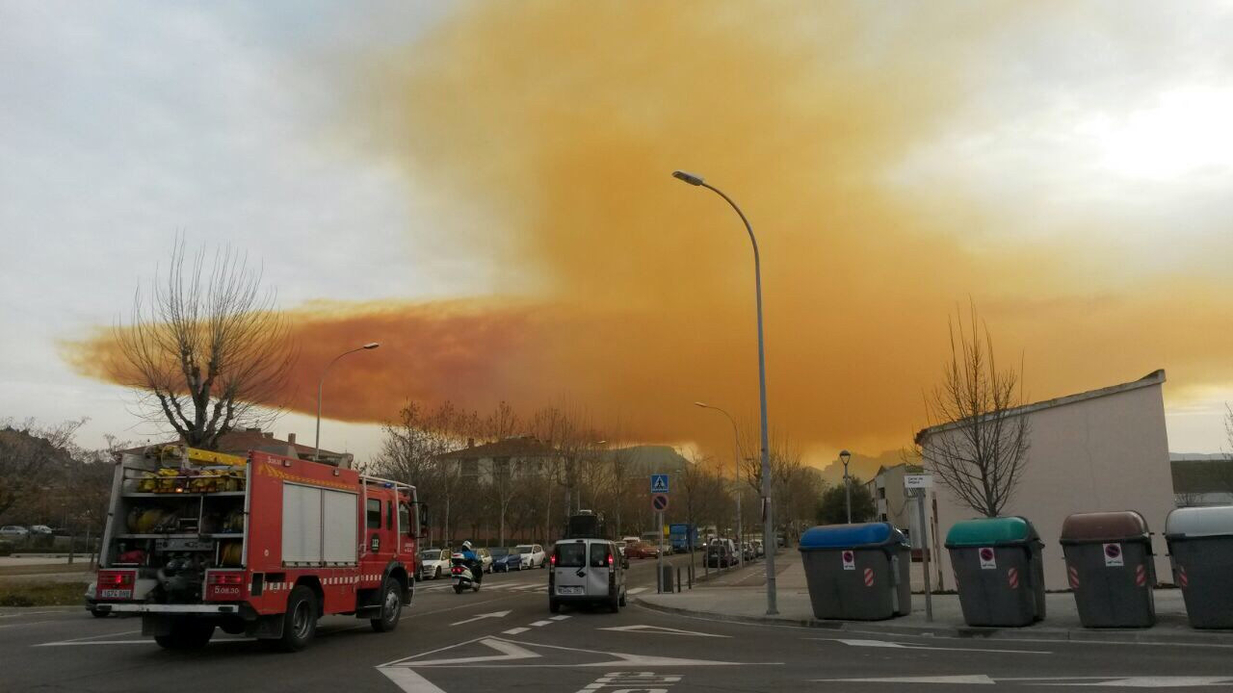
\includegraphics[width=\textwidth]{igualada}
			\caption*{Igualada (2015)}
		\end{subfigure}
		\hfill
		\begin{subfigure}[b]{0.3\textwidth}
			\centering
			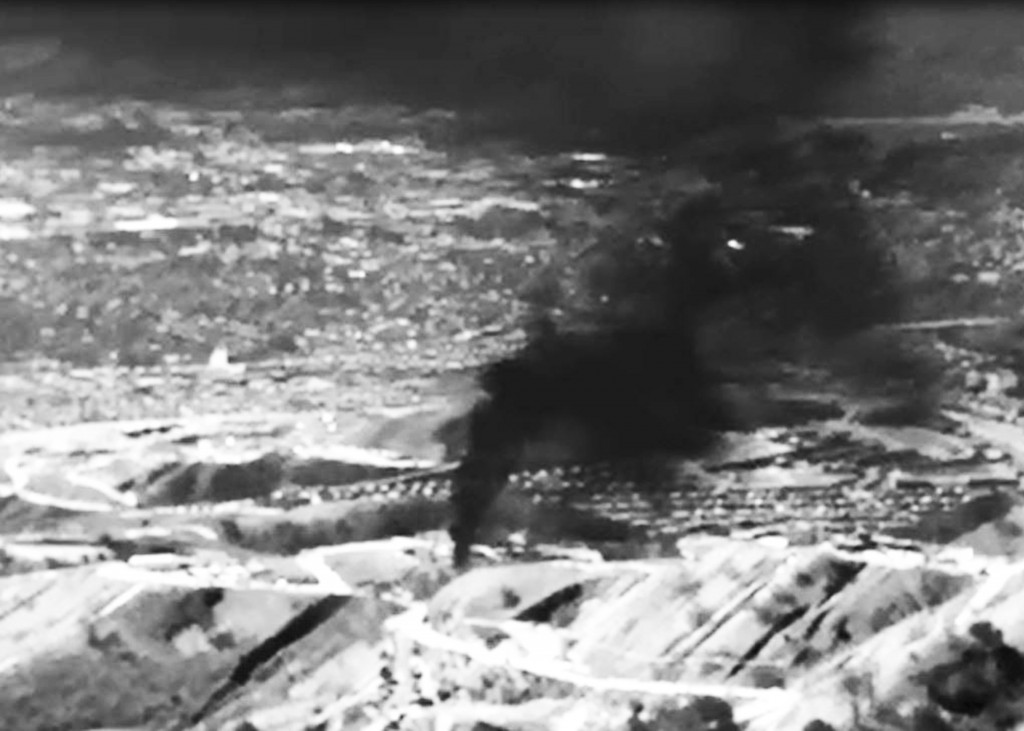
\includegraphics[width=\textwidth]{los_angeles}
			\caption*{Los Angeles (2015)}
		\end{subfigure}
	\end{figure}
	
	Durant de tels événements, les priorités sont alors:
	\begin{itemize}
		\item la mise en sécurité des populations,
		\item l'action des premiers secours pour atténuer/neutraliser le risque.
	\end{itemize}
\end{frame}

% ===== Contexte (2) ================================================================

\begin{frame}
	\frametitle{Contexte}
	Outils pour détecter et évaluer le risque:
	\begin{itemize}
		\item données d'observation (capteurs)
		\item outils de modélisation des phénomènes atmosphériques
	\end{itemize}
	\begin{figure}
		\centering
		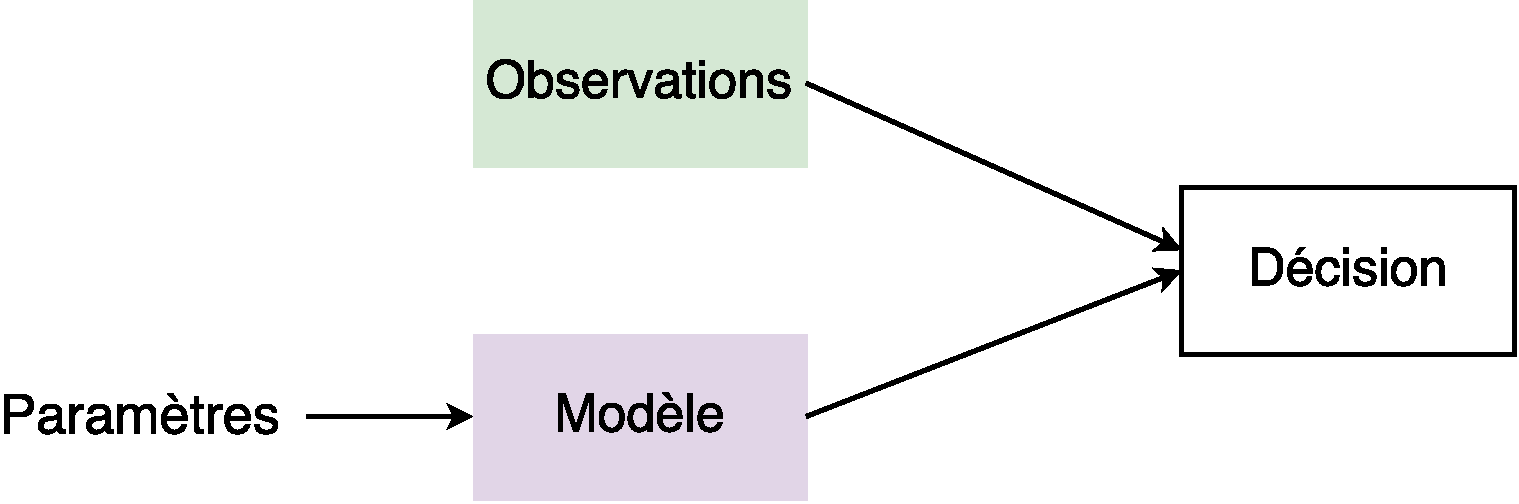
\includegraphics[width=0.9\textwidth]{diagram_context_2.pdf}
	\end{figure}
\end{frame}

% ===== Physique de l'atmosphère ================================================================

\begin{frame}
	\frametitle{Dispersion atmosphérique}
	\begin{block}{Modèle de dispersion}
		Outil de calcul numérique permettant de simuler la propagation dans l'atmosphère d'un rejet de polluant.
	\end{block}
	
	
	Typologie des modèles selon:
	\begin{itemize}
		\item  l'échelle (locale, régionale, synoptique),
		\item le degré de simplification des équations de la mécanique des fluides
	\end{itemize}
	
	Paramètres d'entrée:
	\begin{itemize}
		\item données météorologiques: vent (direction + vitesse), température, humidité, nébulosité, flux de rayonnement...
		\item terme source: position, quantités émises, durée, substance émise...
	\end{itemize}
\end{frame}

% =====  Terme source  ================================================================
\begin{frame}
	\frametitle{Terme source}

\end{frame}


\begin{frame}
	\frametitle{Contexte}
	Accidents + introduire la physique de l'atmo.
\end{frame}
\begin{frame}
	\frametitle{Physique de l'atmosphère}
	Que veut-on modéliser? Quels modèles? (gaussien, eulérien, lagrangien) Quels paramètres? (météo, source)
\end{frame}
\begin{frame}
	\frametitle{Estimer la source: un problème inverse}
	Présenter la dualité direct/inverse. Définir les paramètres d'une source. Transition vers l'état de l'art
\end{frame}
\begin{frame}
	\frametitle{Estimer la source: état de l'art}
	Présenter la question comme un problème inverse mal-posé. Lister les méthodes:
	\begin{itemize}
		\item rétro-transport (x1),
		\item formulation linéaire (minimiser une fonction-coût, maximiser une vraisemblance/posterior): x1= optimisation+ reg., x1 = : max likelihood + prior, lier en couleur avec la slide précédente
		\item formulation générale: équation, dire qu'on veut trouver les paramètres $x_s$ et $q$ au lieu de reconstruire le vecteur $\varsigma$. Génétique: OK car problème d'exploration combinatoire difficile (schéma?) Bayésien et simulation stochastique: explorer efficacement l'espace des paramètres par échantillonnage aléatoire.
	\end{itemize} 
\end{frame}
\begin{frame}
	\frametitle{Problématique de recherche}
	\begin{itemize}
		\item le choix bayésien: pourquoi?
		\item Comment? C'est le coeur de la thèse. Poser la problématique.
	\end{itemize}
\end{frame}
\section{Inférence bayésienne et méthodes de Monte-Carlo}
\begin{frame}
	(vide)
\end{frame}
\section{Application au cas expérimental FFT07}
\begin{frame}
	(vide)
\end{frame}
\section{Application avec modèle rétrograde aux cas simulés Beaune et Opéra}
\begin{frame}
	(vide)
\end{frame}
\section{Conclusions et perspectives}
\begin{frame}
	(vide)
\end{frame}
\end{document}
